\subsection{\href{http://www.wolfcut.es/}{Wolfcut}}
   \hypertarget{subsec:wolfcut}
   Se desarrolló un sistema embebido para el control on line de una máquina que utiliza un controlador autónomo NK105 que no cuenta con capacidades de control remoto.\\
   Se utilizó una computadora embebida \textit{beagle bone green wireless} que se comporta como un USB mass storage para el intercambio de archivos con el controlador sin necesidad de conectar y desconectar un pendrive.\\
   Se intercaló con el cableado del mando manual una placa que permite enviar comandos al controlador emulando el funcionamiento del comando.\\
   Dentro del embebido se corre un sistema linux compilado expresamente utilizando un cross compiler compilado para arm, se compilo el kernel, un filesystem utilizando build root y se ajustó el sistema configFS para que el embebido se comporte como mass storage y finalmente se implemento una pagina web sobre apache con php para la interacción del usuario tanto desde una PC o desde un móvil.
   En la figura \ref{fig:wolfcut_capas} se puede ver el modelo de capas implementado y la pagina web de control.
     \begin{figure}
      \begin{center}
         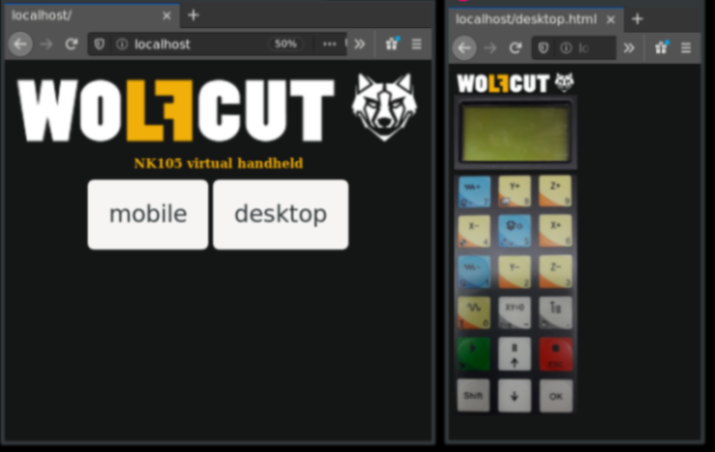
\includegraphics[width=0.3\textwidth]{wolfcut1.png}
         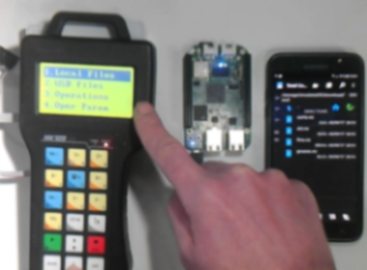
\includegraphics[width=0.3\textwidth]{wolfcut2.png}
         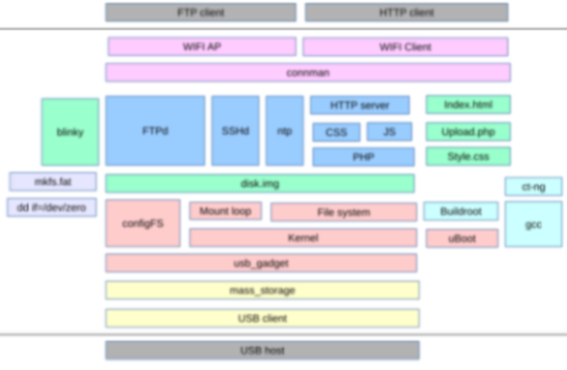
\includegraphics[width=0.3\textwidth]{wolfcut3.png}
      \end{center}
      \caption{Modelo de capas de software y pagina web para controlar remotamente una maquina CNC mediante la intervencion de un controlador NK105.}
      \label{fig:wolfcut_capas}
   \end{figure}

   En las figuras \ref{fig:wolfcut_implementacion} se pueden ver capturas del sistema de compilación.

     \begin{figure}
      \begin{center}
         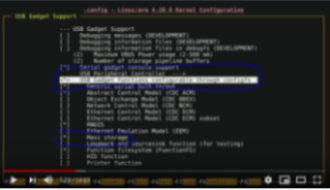
\includegraphics[width=0.3\textwidth]{wolfcut4.png}
         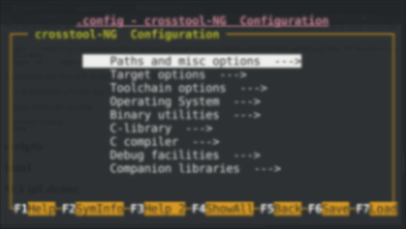
\includegraphics[width=0.3\textwidth]{wolfcut5.png}
         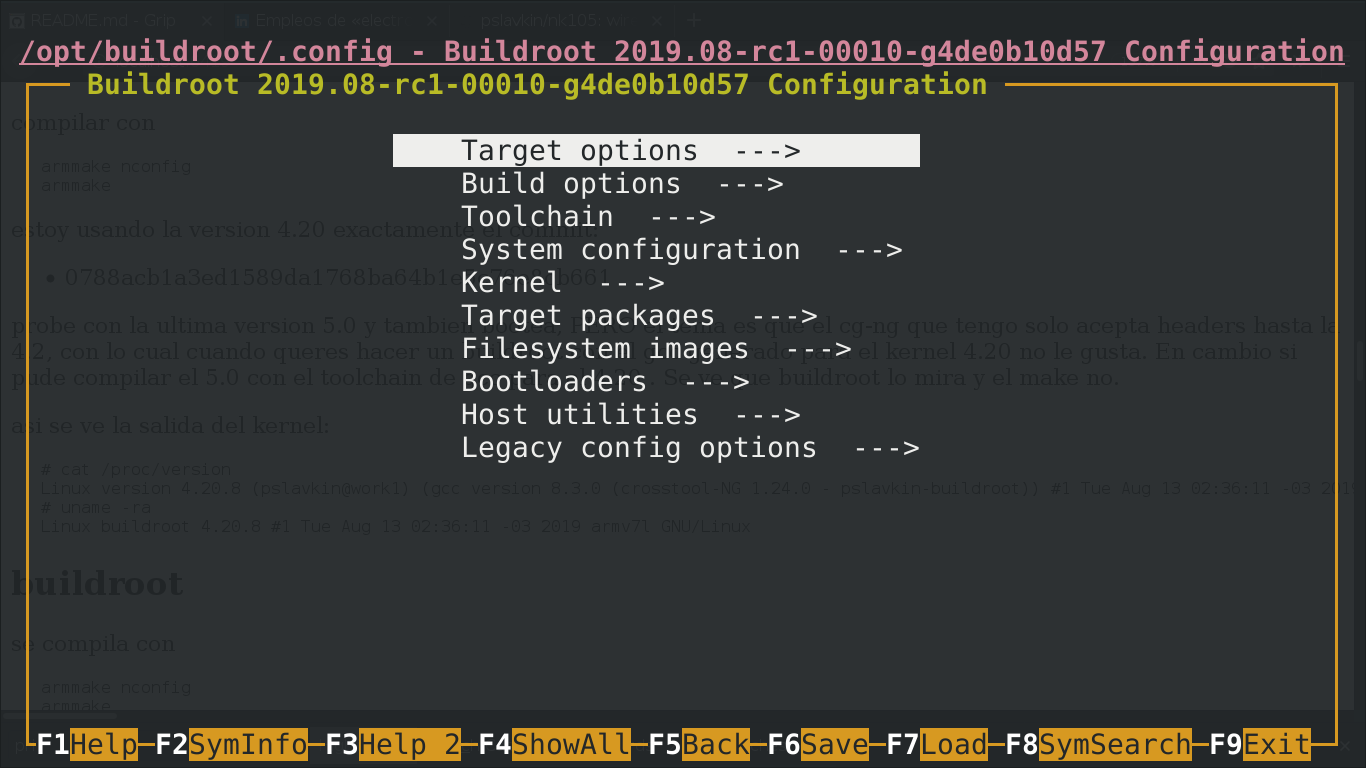
\includegraphics[width=0.3\textwidth]{wolfcut6.png}
      \end{center}
      \caption{Compilación de cross-tool con ng, kernel con gcc y file system con buildroot}
      \label{fig:wolfcut_implementacion}
   \end{figure}
